\documentclass[tikz,border=2pt]{standalone}
\usepackage{amsmath,amssymb}
% sans serif for text and math
\renewcommand{\familydefault}{\sfdefault}
\usepackage[eulergreek]{sansmath}
\sansmath
\usetikzlibrary{positioning,arrows.meta}
\definecolor{popteal}{HTML}{5BC5D0}
\definecolor{sampgray}{HTML}{7F7F7F}

\begin{document}
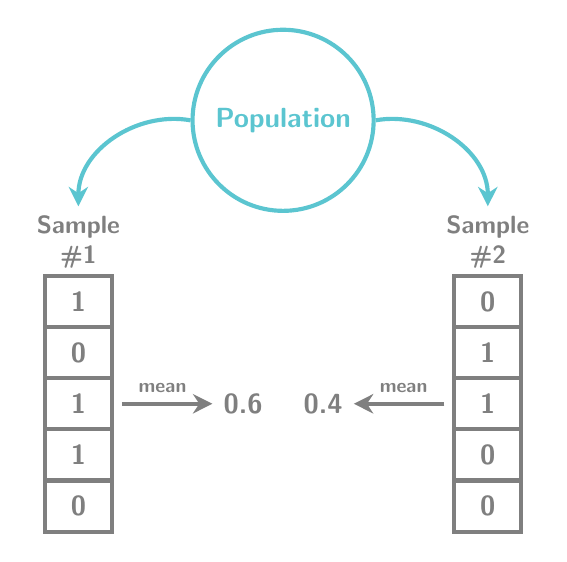
\begin{tikzpicture}[
    font=\bfseries,
    cell/.style={draw=sampgray, line width=1.5pt, text=sampgray,
      minimum width=0.85cm, minimum height=0.65cm, inner sep=0pt},
    lab/.style={text=sampgray, align=center, font=\bfseries\small},
    arr/.style={-{Stealth[length=7pt, width=7pt]}, line width=1.5pt}
  ]
  % population
  \node[circle, draw=popteal, line width=1.5pt, text=popteal,
    minimum size=2.3cm] (pop) at (0,0) {Population};

  % samples: one column of cells per sample
  \foreach \side/\x/\num/\vals in {L/-2.6/1/{1,0,1,1,0}, R/2.6/2/{0,1,1,0,0}} {
    \node[lab] (lab\side) at (\x,-1.55) {Sample\\\#\num};
    \foreach \v [count=\i] in \vals {
      \node[cell] (\side\i) at (\x, {-2.3 - 0.65*(\i-1)}) {\v};
    }
  }

  % population -> samples
  \draw[arr, draw=popteal] (pop.west) to[out=170, in=90] (labL.north);
  \draw[arr, draw=popteal] (pop.east) to[out=10, in=90] (labR.north);

  % sample means
  \draw[arr, draw=sampgray] (L3.east) ++(0.1,0) -- ++(1.15,0)
    node[pos=0.45, above, lab, font=\bfseries\scriptsize] {mean}
    node[right, text=sampgray] {0.6};
  \draw[arr, draw=sampgray] (R3.west) ++(-0.1,0) -- ++(-1.15,0)
    node[pos=0.45, above, lab, font=\bfseries\scriptsize] {mean}
    node[left, text=sampgray] {0.4};
\end{tikzpicture}
\end{document}
